\documentclass[12pt]{report}
\usepackage[utf8]{inputenc}
\usepackage[russian]{babel}
%\usepackage[14pt]{extsizes}
\usepackage{listings}
\usepackage{graphicx}
\usepackage{amsmath,amsfonts,amssymb,amsthm,mathtools} 
\usepackage{pgfplots}
\usepackage{filecontents}
\usepackage{indentfirst}
\usepackage{eucal}
\usepackage{float}
\usepackage{amsmath}
\usepackage{enumitem}
\frenchspacing

\usepackage{indentfirst} % Красная строка


%\usetikzlibrary{datavisualization}
%\usetikzlibrary{datavisualization.formats.functions}

\usepackage{amsmath}


% Для листинга кода:
\lstset{ %
	language=haskell,                 % выбор языка для подсветки (здесь это С)
	basicstyle=\small\sffamily, % размер и начертание шрифта для подсветки кода
	numbers=left,               % где поставить нумерацию строк (слева\справа)
	numberstyle=\tiny,           % размер шрифта для номеров строк
	stepnumber=1,                   % размер шага между двумя номерами строк
	numbersep=5pt,                % как далеко отстоят номера строк от подсвечиваемого кода
	showspaces=false,            % показывать или нет пробелы специальными отступами
	showstringspaces=false,      % показывать или нет пробелы в строках
	showtabs=false,             % показывать или нет табуляцию в строках
	frame=single,              % рисовать рамку вокруг кода
	tabsize=2,                 % размер табуляции по умолчанию равен 2 пробелам
	captionpos=t,              % позиция заголовка вверху [t] или внизу [b] 
	breaklines=true,           % автоматически переносить строки (да\нет)
	breakatwhitespace=false, % переносить строки только если есть пробел
	escapeinside={\#*}{*)}   % если нужно добавить комментарии в коде
}

\usepackage[left=2cm,right=2cm, top=2cm,bottom=2cm,bindingoffset=0cm]{geometry}
% Для измененных титулов глав:
\usepackage{titlesec, blindtext, color} % подключаем нужные пакеты
\definecolor{gray75}{gray}{0.75} % определяем цвет
\newcommand{\hsp}{\hspace{20pt}} % длина линии в 20pt
% titleformat определяет стиль
\titleformat{\chapter}[hang]{\Huge\bfseries}{\thechapter\hsp\textcolor{gray75}{|}\hsp}{0pt}{\Huge\bfseries}


% plot
\usepackage{pgfplots}
\usepackage{filecontents}
\usetikzlibrary{datavisualization}
\usetikzlibrary{datavisualization.formats.functions}

\begin{document}
	%\def\chaptername{} % убирает "Глава"
	\thispagestyle{empty}
	\begin{titlepage}
		\noindent \begin{minipage}{0.15\textwidth}
			
\includegraphics[width=\linewidth]{b_logo}
		\end{minipage}
		\noindent\begin{minipage}{0.9\textwidth}\centering
			\textbf{Министерство науки и высшего образования Российской Федерации}\\
			\textbf{Федеральное государственное бюджетное образовательное учреждение высшего образования}\\
			\textbf{~~~«Московский государственный технический университет имени Н.Э.~Баумана}\\
			\textbf{(национальный исследовательский университет)»}\\
			\textbf{(МГТУ им. Н.Э.~Баумана)}
		\end{minipage}
		
		\noindent\rule{18cm}{3pt}
		\newline\newline
		\noindent ФАКУЛЬТЕТ $\underline{\text{«Информатика и системы управления»}}$ \newline\newline
		\noindent КАФЕДРА $\underline{\text{«Программное обеспечение ЭВМ и информационные технологии»}}$\newline\newline\newline\newline\newline
		
		
		\begin{center}
			\noindent\begin{minipage}{1.3\textwidth}\centering
				\Large\textbf{  Отчёт по лабораторной работе №7}\newline
				\textbf{по дисциплине "Анализ алгоритмов"}\newline\newline
			\end{minipage}
		\end{center}
		
		\noindent\textbf{Тема} $\underline{\text{Поиск в словаре}}$\newline\newline
		\noindent\textbf{Студент} $\underline{\text{Романов А.В.}}$\newline\newline
		\noindent\textbf{Группа} $\underline{\text{ИУ7-53Б}}$\newline\newline
		\noindent\textbf{Преподаватели} $\underline{\text{Волкова Л.Л., Строганов Ю.В.}}$\newline\newline\newline
		
		\begin{center}
			\vfill
			Москва~---~\the\year
			~г.
		\end{center}
	\end{titlepage}
	
	
	\tableofcontents
	
\newpage
\chapter*{Введение}
\addcontentsline{toc}{chapter}{Введение}
	
Словарь  -- структура данных, построенная  на  основе  пар  значений.  Первое  значение  пары -- ключ  для идентификации элементов, второе  -- собственно сам хранимый элемент. Например, в телефонном справочнике номеру  телефона  соответствует  фамилия  абонента. Существует несколько основных различных реализаций словаря: массив, двоичные деревья поиска, хеш-таблицы. Каждая из этих реализаций имеет свои минусы и плюсы, например время поиска, вставки и удаления элементов.
	
\section*{Цель лабораторной работы}
	
Целью данной лабораторной работы является изучение алгоритмов поиска в словаре.
	
\section*{Задачи лабораторной работы}
	
В рамках выполнения работы необходимо решить следующие задачи:
	
\begin{itemize}
	\item реализовать три алгоритма поиска в словаре;
	\item замерить и сравнить время выполнения алгоритмов;
	\item сделать выводы на основе проделанной работы.
\end{itemize}
	
\chapter{Аналитическая часть}
	
В данном разделе представленные теоретические сведения о рассматриваемых алгоритмах.
	
\section{Полный перебор}
	
Алгоритм полного перебора заключается в проходе по словарю, до того момента, пока не будет найден искомый ключ. В рассматриваемом алгоритме возможно $N + 1$ случаев расположения ключа: ключ является $i$-ым элементом словаря либо его нет в словаре в принципе. 
	
Лучший случай (трудоемкость $O(1)$): ключ расположен в самом начале словаря и найден за одно сравнение). Худший случай (трудоемкость $O(N)$): ключ расположен в самом конце словаря либо ключ не находится в словаре.
	
\section{Двоичный поиск}
	
Данный алгоритм подходит только для заранее упорядоченного словаря.
	
Процесс двоичного поиска можно описать следующим образом: 
	
\begin{itemize}
	\item получить значение находящееся в середине словаря и сравнить его с ключом;
	\item в случае, если ключ меньше данного значения, продолжить поиск в младшей части словаря, в обратном случае -- в старшей части словаря;
	\item на новом интервале снова получить значение из середины этого интервала и сравнить с ключом.
	\item поиск продолжать до тех пор, пока не будет найден искомый ключ, или интервал поиска не окажется пустым.
\end{itemize}
	
Обход словаря данным алгоритм можно представить в виде дерева, поэтому трудоемкость в худшем случае составит $\log_{2}{N}$. Можно сделать вывод, что алгоритм двоичного поиска работает быстрее чем алгоритм полного перебора, но при этом требует предварительной обработки данных (сортировки).
	
\section{Частотный анализ}
	
Данный алгоритм также требует предварительной обработки данных, а именно:
	
\begin{itemize}
	\item упорядочить словарь;
	\item разбить словарь на сегменты.
\end{itemize}
	
Словарь разбивается на сегменты по какому-либу признаку и сортируется по частоте. Например, если ключ является строкой, то можно сделать разбиение по первой букве в ключе. Если ключ является целым числом, можно провести разбиение по остатку от деления ключа на некоторое число $K$.
	
После выполнения разбиения, нужно определить к какому сегменту относится искомый ключ и провести на этом сегменте двоичный поиск.
	
Таким образом, время поиска в словаре увеличивается (особенно для самых часто встречаемых ключей), но, при этом, так же как и алгоритм двоичного поиска, частотный анализ требует предварительной обработки данных. 
	
\section{Описание словаря}
	
Ключом в рассматриваемом мною словаре является ID преподавателя, а значением количество часов, которые он тратит на проведение лабораторных работ. Оба значения являются целочисленными. Так как значение ключа является целым числом, деление на сегменты будет производится посредствам получением остатка от деления ключа на некоторое число $K$.
	
\section*{Вывод}
В данном разделе были рассмотренны особенности алгоритмов поиска в словаре.
	
\chapter{Конструкторская часть}
	
В данном разделе представлены схемы рассматриваемых алгоритмов.
	
\section{Разработка алгоритмов}
	
На рисунках 2.1 - 2.3 приведены схема алгоритмов поиска в словаре.
	
	\begin{figure}[H]
		\centering
		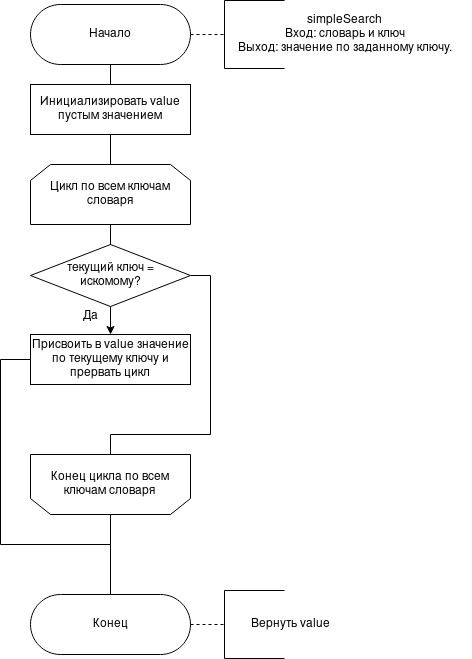
\includegraphics[scale=0.62]{simple_search.jpg}
		\caption{Схема алгоритма полного перебора.}
		\label{fig:mpr}
	\end{figure}
	
	\begin{figure}[H]
		\centering
		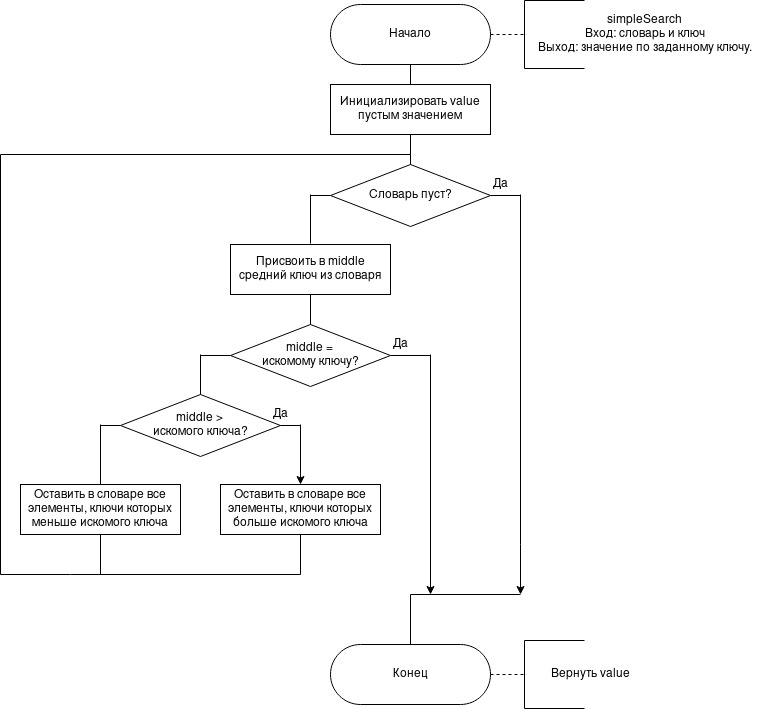
\includegraphics[scale=0.7]{binary_search.jpg}
		\caption{Схема алгоритма двоичного поиска.}
		\label{fig:mpr}
	\end{figure}
	
	\begin{figure}[H]
		\centering
		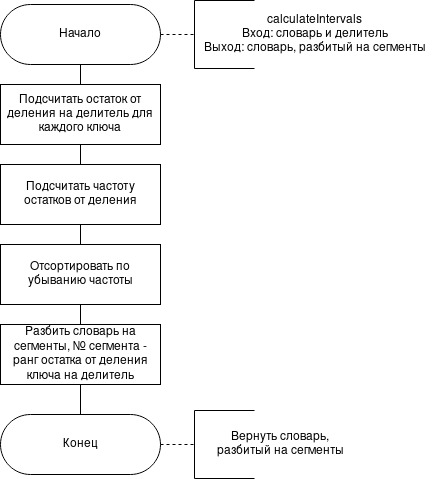
\includegraphics[scale=1]{calculate_intervals.jpg}
		\caption{Схема алгоритма частотного анализа.}
		\label{fig:mpr}
	\end{figure}

	\begin{figure}[H]
		\centering
		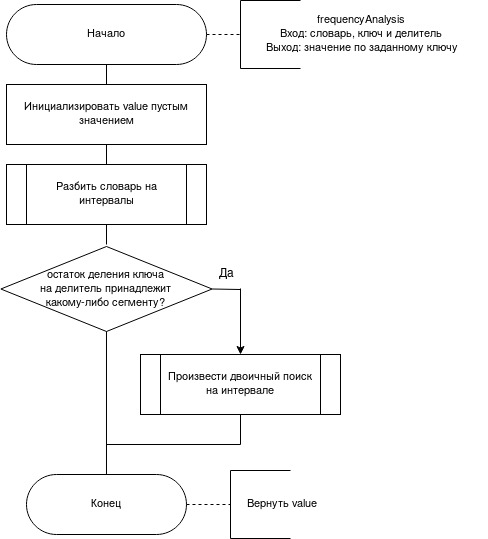
\includegraphics[scale=1]{freq_analysis.jpg}
		\caption{Схема алгоритма поиска с использованием частотного анализа.}
		\label{fig:mpr}
	\end{figure}
	
	
	\section*{Вывод}
	
	На основе теоретических данных, полученных аз аналитического раздела, были построенны схемы алгоритмов поиска в словаре.
	
	\chapter{Технологическая часть}
	
	В данном разделе приведены средства реализации и листинги кода.
	
	\section{Требование к ПО}
	
	К программе предъявляется ряд требований:
	
	\begin{itemize}
		\item на вход подается текстовый файл содержащий пары вида: ID преподавателя -- количество часов потраченных на проведение лабораторных работ, кроме этого, с клавиатуры считывается искомый в словаре ключ (ID преподавателя);
		\item на выходе -- значение для введенного с клавиатуры ключа.
	\end{itemize}
	
	\section{Средства реализации}
	
	Для реализации ПО я выбрал язык программирования Haskell \cite{Haskell}. Данный выбор обусловлен моим желанием расширить свои знания в области применения данного языка программирования.
	
\section{Реализация алгоритмов}

В листингах 3.1 - 3.3 представлены листинги алгоритмов поиска в словаре.
	
\begin{lstlisting}[label=some-code,caption=Алгоритм полного перебора, language=Haskell]
simpleSearch :: (Ord a, Eq b) => V.Vector (a, b) -> a -> Maybe b
simpleSearch dict key = simpleSearch' dict key $ V.head dict 
  where
    simpleSearch' dict key curr | key == fst curr = Just $ snd curr
    simpleSearch' dict key curr | V.null dict = Nothing
    simpleSearch' dict key curr | otherwise = simpleSearch' (V.tail dict) key $ V.head dict
\end{lstlisting}
	
\begin{lstlisting}[label=some-code,caption=Алгоритм двоичного поиска, language=Haskell]
binarySearch :: (Ord a, Eq b) => V.Vector (a, b) -> a -> Maybe b 
binarySearch dict key = binarySearch' dict key $ middle dict
  where
    droppedSize dict = if V.length dict >= 2 then V.length dict else 2
    fstHalf dict = V.take ((V.length dict) `div` 2) dict
    sndHalf dict = V.drop ((droppedSize dict) `div` 2) dict
    middle dict = dict V.! ((V.length dict) `div` 2)

	binarySearch' dict key curr | V.null dict = Nothing
	binarySearch' dict key curr | key == fst curr = Just $ snd curr
	binarySearch' dict key curr | key > fst curr = binarySearch' (sndHalf dict) key (middle $ sndHalf dict)
	binarySearch' dict key curr | key <= fst curr = binarySearch' (fstHalf dict) key $ (middle $ fstHalf dict)
\end{lstlisting}

\begin{lstlisting}[label=some-code,caption=Алгоритм поиска с использованием частотного анализа, language=Haskell]
calculateIntervals :: Eq b => V.Vector (Int, b) -> Int -> V.Vector (V.Vector (Int, b))
calculateIntervals dict divider = intervals
  where 
    remainder = V.foldl (\acc x -> acc V.++ (V.fromList [(fst x `mod` divider, x)])) (V.empty) dict
    intervals = V.foldl (
      \acc x ->
        acc V.// [(fst x, acc V.! (fst x) V.++ V.fromList [snd x])])
          (V.generate divider (\x -> V.empty)) remainder


frequencyAnalysis :: Eq b => V.Vector (Int, b) -> Int -> Int -> Maybe b
frequencyAnalysis dict key divider = 
  if V.null $ disiredInterval key divider
  then Nothing 
  else binarySearch (disiredInterval key divider) key
    where
      intervals = calculateIntervals dict divider
      disiredInterval k d = intervals V.! (k `mod` d)
\end{lstlisting}
	
	
\section{Тестовые данные}

В таблице 3.1 приведены тестовые данные, где ПП -- полный перебор, ДП -- двоичный поиск, ЧА -- частотный анализ. Все тесты были пройденны успешно.

\begin{table}[H]
	\caption{Таблица тестовых данных алгоритмов поиска в словаре.}

	\begin{center}

		\begin{tabular}{|c c c c c|} 

			\hline

			Входные данные & Ожидаемый результат & ПП & ДП & ЧА \\  

			\hline

			1 & 217 & 217 & 217 & 217 \\

			\hline

			145 & 338 & 338 & 338 & 338 \\

			\hline

			876 & 111 & 111 & 111 & 111 \\

			\hline

			1002 & Нет ключа & Нет ключа & Нет ключа & Нет ключа \\
			\hline
		\end{tabular}

	\end{center}

\end{table}
	
\section*{Вывод}
	
В данном разделе была разработаны и протестированны алгоритмы поиска в словаре.
	
\chapter{Исследовательская часть}
	
В данном разделе приведен анализ характеристик разработанного ПО.

\section{Технические характеристики}
	
Ниже приведены технические характеристики устройства, на котором было проведено тестирование ПО:
	
\begin{itemize}
	\item Операционная система: Debian \cite{debian} Linux \cite{linux} 11 <<bullseye>> 64-bit.
	\item Оперативная память: 12 GB.
	\item Процессор: Intel(R) Core(TM) i5-3550 CPU @ 3.30GHz \cite{i5}.	
\end{itemize}
	
\section{Время выполнения алгоритмов}
	
Время выполнения алгоритма замерялось с помощью применения технологии профайлинга \cite{profiling}. Данный инструмент даёт детальное описание количество вызовов и количества времени CPU, затраченного на выполнение каждой функции.

В таблице 4.1 приведено сравнение времени выполнения алгоритмов: минимальное время поиска, среднее время поиска, максимальное время поиска.

\begin{table} [H]
		\caption{Таблица времени выполнения алгоритмов поиска в словаре (в секундах)}
		\begin{center}
			\begin{tabular}{|c c c c |} 
				\hline
				Размер словаря & Полный перебор & Двоичный поиск & Частотный анализ  \\  
				\hline
				1000 & (0.01, 0.05, 0.1) & (0.01, 0.015, 0.02) & (0.01, 0.018, 0.021)  \\
				\hline
				10000 & (0.01, 0.49, 1.02) & (0.01, 0.05, 0.2) & (0.01, 0.047, 0.19) \\
				\hline
				100000 & (0.01, --, --) & (0.01, 0.1, 0.51) & (0.01, 0.095, 0.17) \\
				\hline
			\end{tabular}
		\end{center}
\end{table}
	
\section*{Вывод}
	
Алгоритм двоичного поиска превосходит алгоритм полного перебора на всех размерах словаря (на которых проводилось тестирование). Например, при размере словаря 10000 ключей, двоичный поиск в среднем случае работает в 100 раз быстрее. 
Алгоритм поиска с использованием частотного анализа начинает выигрывать у алгоритма двоичного поиска при увеличении размера словаря. Так, например, при размере словаря 100000 ключей, в среднем случае такой алгоритм работает быстрее в 1.08 раз, в сравнении с двоичным поиском. 
Минимальное возможное время поиска в словаре для всех алгоритмов примерно одинаково на всех размерах словаря.

\chapter*{Заключение}
\addcontentsline{toc}{chapter}{Заключение}
	
В рамках данной лабораторной работы лабораторной работы была достигнута её цель: изучены алгоритмы поиска в словаре. Также выполнены следующие задачи:
	
\begin{itemize}
	\item реализованны три алгоритма поиска в словаре;
	\item замерено время выполнения алгоритмов;
	\item сделаны выводы на основе проделанной работы;
\end{itemize}

В результате проведения сравнения скорости выполнения алгоритмов, можно сделать вывод, что алгоритм поиска с использование частотного анализа начинает выигрывать у алгоритма двоичного поиска на больших размерах словарей. Так, например, при размере словаря в 100000 ключей, алгоритм работает в среднем случае быстрее в 1.08 раз. 

Стоит отметить, что и алгоритм двоичного поиска, и алгоритм поиска с использованием частотного анализа требуют предварительный обработки данных (сортировки и разбиение на сегменты соотвественно), в отличие от алгоритма полного перебора. Но именно это позволяет стать этим алгоритмам намного эффективнее в сравнении с алгоритмом полного перебора.

\addcontentsline{toc}{chapter}{Литература}
\bibliographystyle{utf8gost705u}  % стилевой файл для оформления по ГОСТу
\bibliography{51-biblio}          % имя библиографической базы (bib-файла)
	
\end{document}
